\section{Partie \emph{user guide}}
\label{sec:user-guide}

\par L’interface graphique est très facile de prise en main.
\par Une bonne utilisation de l'application passe naturellement par un tutoriel expliquant les diverses fonctionnalités de cette dernière.

\paragraph{Lancement de l'application et connexion au serveur Supélec}
\label{sec:lancement_app}

\par Au lancement de l’application, l’IU de connexion figure \ref{fig:iucon_launch} se lance.

\begin{figure}[h!]
  \centering
  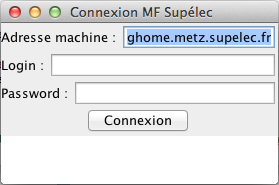
\includegraphics[width=6cm]{images/iuconnexion_launch.png}
  \caption{IU de connexion au lancement de l'application}
  \label{fig:iucon_launch}
\end{figure}

\par L’utilisateur doit renseigner l’adresse de la machine frontale sur laquelle il souhaite se connecter (la valeur par défaut est ghome.metz.supelec.fr), son login ainsi que son mot de passe comme réalisé à la figure \ref{fig:iucon_connect}.

\begin{figure}[h!]
  \centering
  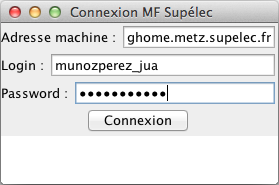
\includegraphics[width=6cm]{images/iuconnexion_connect.png}
  \caption{IU de connexion au lancement de l'application}
  \label{fig:iucon_connect}
\end{figure}

\par L’appui sur le bouton \emph{Connexion} lance l’identification auprès du serveur Supélec. Si l'authentification est valide, l'IU de connexion se ferme et l'IU d'allocation apparaît.

\paragraph{Allocation de noeuds : création d'un job}

\par La figure \ref{fig:iualloc_launch} représente l'IU d'allocation.

\begin{figure}[h!]
  \centering
  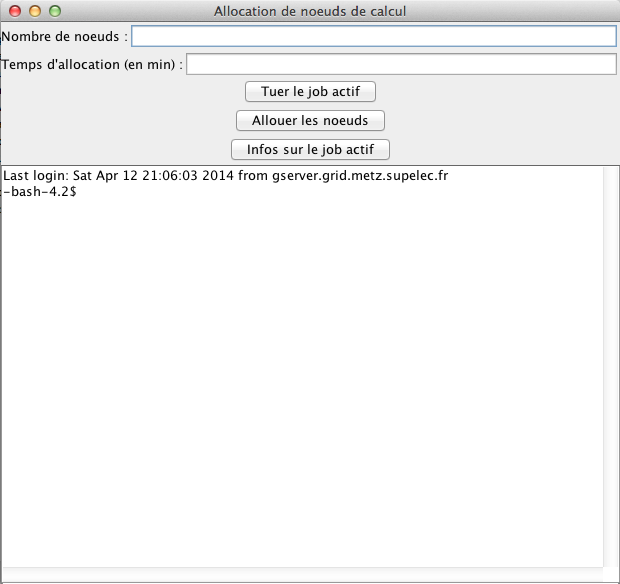
\includegraphics[width=11cm]{images/iuallocation_launch.png}
  \caption{IU d'allocation après validation de l'authentification}
  \label{fig:iualloc_launch}
\end{figure}

\par À ce stade il est désormais possible d'allouer des noeuds de calcul. Pour ce faire, l'utilisateur doit renseigner le nombre de noeuds souhaités (un entier naturel) ainsi que le temps d'allocations (en minutes). Après appui sur le bouton \emph{Allouer des noeuds}, l'IU d'allocation ressemble à la figure \ref{fig:iualloc_nodes}.

\begin{figure}[h!]
  \centering
  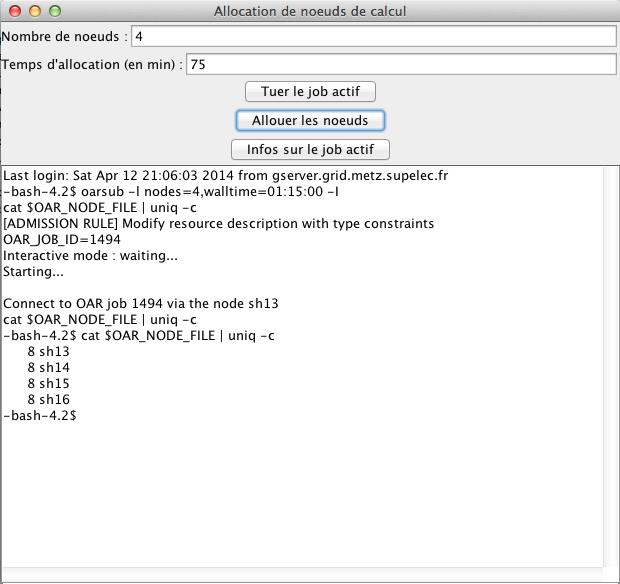
\includegraphics[width=11cm]{images/iuallocation_ask_nodes.png}
  \caption{IU d'allocation : allocation de noeuds}
  \label{fig:iualloc_nodes}
\end{figure}

\par Nous pouvons voir que le job correspondant à notre requête est le job numéro 1494. La machine de référence est le nœud sh13 (machine du cluster Skynet). Les nœuds qui nous sont alloués pour une durée de 75 minutes sont sh13 (8), sh14 (8), sh15 (8) et sh16 (8). Le nombre entre parenthèses correspond au nombre de cœurs processeurs que possède la machine. D’un cluster à l’autre il se peut que ce nombre varie. Pour indication, les machines du cluster Cameron possèdent 6 cœurs alors que celles d’InterCel n’en possèdent que 2.

\paragraph{Informations sur le job}
\label{sec:info_job}

\par Le job étant actif il est possible d'obtenir des informations sur l'identifiant du job, le temps d'allocation restant, les ressources qui ont été assignées et bien d'autres.
\par L'appui sur le bouton \emph{Infos sur le job actif} nous renvoie sur la fenêtre le message ci dessous.

\begin{verbatim}
-bash-4.2$ oarstat -fj $OAR_JOB_ID
Job_Id: 1494
    job_array_id = 1494
    job_array_index = 1
    name = 
    project = default
    owner = munozperez_jua
    state = Running
    wanted_resources = -l "{type = 'default'}/network_address=4,walltime=1:15:0" 
    types = 
    dependencies = 
    assigned_resources = 105+106+107+108+109+110+111+112+113+114+115+
116+117+118+119+120+121+122+123+124+125+126+127+128+129+130+131+132+
133+134+135+136
    assigned_hostnames = sh13+sh14+sh15+sh16
    queue = default
    command = 
    launchingDirectory = /usr/users/promo2015/munozperez_jua
    stdout_file = OAR.1494.stdout
    stderr_file = OAR.1494.stderr
    jobType = INTERACTIVE
    properties = desktop_computing = 'NO'
    reservation = None
    walltime = 1:15:0
    submissionTime = 2014-04-12 21:53:53
    startTime = 2014-04-12 21:53:54
    cpuset_name = munozperez_jua_1494
    initial_request = oarsub -l nodes=4,walltime=01:15:00 -I
    message = R=32,W=1:15:0,J=I (Karma=0.815)
    scheduledStart = 2014-04-12 21:53:54
    resubmit_job_id = 0
    events = 
\end{verbatim}

\par Il sera possible à tout moment, tant qu'il y a un job actif, de suivre l'évolution du job. 

\paragraph{Tuer le job}
\label{sec:tuer_job}

\par Si jamais l'utilisateur s'est trompé dans le nombre de noeuds ou le temps d'allocation lors de la création de son job, il est possible de revenir en arrière en tuant ledit job. Pour ce faire, il suffit d'appuyer sur le bouton \emph{Tuer le job actif}.
\par La figure \ref{fig:iualloc_kill} montre le message renvoyé par le serveur après exécution de la commande. 

\begin{figure}[h!]
  \centering
  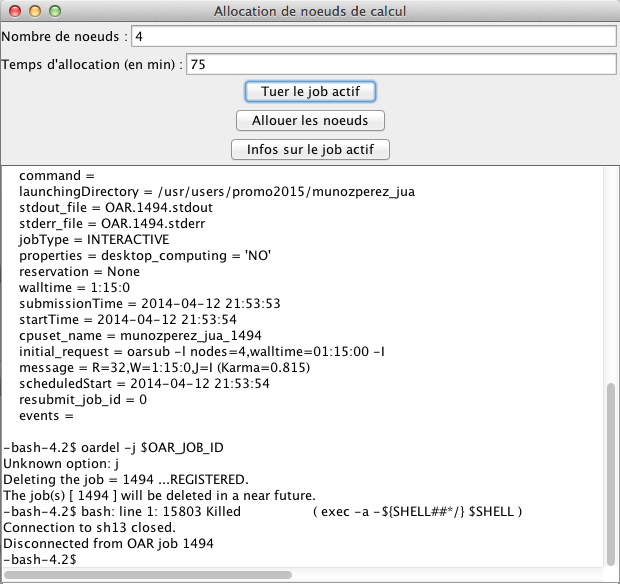
\includegraphics[width=11cm]{images/iuallocation_kill_job.png}
  \caption{IU d'allocation : tuer le job}
  \label{fig:iualloc_kill}
\end{figure}

\par Éliminer le job actif 1494 consiste tout simplement pour \emph{OAR} à fermer la connexion à la machine de référence, ici sh13.
\par À travers ce tutoriel, nous avons bien vu que l'application implémentée réalise bien les fonctionnalités mentionnées dans les précédentes parties et est très simple d'utilisation.

%%% Local Variables: 
%%% mode: latex
%%% TeX-master: "CompteRendu"
%%% End: 